\chapter{Adding Rodinia to Vortex}

One of \Gls{vortex}' weaknesses is its benchmark suite. Vortex includes only a few benchmarks, all of which are quite small and which behaviours does not match real-world applications. When lacking reasonable benchmarks, it is difficult obtain conclusive results about the performance of \Gls{vortex}. To solve this, I brought Rodinia \cite{rodinia}\cite{rodinia_characterization}, a commonly used set of benchmarks for parallel computing\cite{cactus}, to the Vortex ecosystem. This chapter describes the work done to enable Rodinia benchmarks to run on \Gls{vortex}. 

%\textcolor{red}{Vortex only has a few benchmarks. These programs have quite simple kernels and does not represent the behaviour of real world applications. Rodinia\cite{rodinia}\cite{rodinia_characterization} is a commonly used set of benchmarks for parallel computing \cite{cactus} with an OpenCL version. This chapter describes the work done to run Rodinia benchmarks on \Gls{vortex}}

\section{Reading Performance Data} \label{sec:reading_perf}

All the benchmarks included with \Gls{vortex} executed one kernel once, thus the existing setup for gathering performance data, created by the \Gls{vortex} team, could take advantage of this. \Gls{vortex} utilize internal performance counters to collect performance data. Each \acrshort{sm} has its own counters, which are accessible as addressable \acrshort{csr} registers. Before a kernel is enqueued, the GPU is reset, this includes the performance registers. After the reset, different metrics are collected regarding the execution. When an \acrshort{sm} finish execution of its allocated workload, it ends by reading the relevant \acrshort{csr} registers and writing their contents to memory. The code related to dumping the performance counter to memory is included in every kernel by a stub. At the end of the benchmark, the host can read the memory, and collect and accumulate the performance metrics for the \acrshortpl{sm} individually, and the \acrshort{gpu} as a whole.

Most of the benchmarks in Rodinia has more than one kernel, or executes a single kernel multiple times. When executing a multi-kernel benchmark, only the last execution would be recorded, because the \acrshort{gpu} would reset between kernel executions. Obtaining performance data for all kernels in a benchmark is important as they might possess radically different behaviours. An example of this would be the \textit{streamcluster} benchmark which has two kernels: \textit{memset} and \textit{pgain}. The memset kernel sets global memory to a given value. This results in a short loop and many writes to memory. The pgain kernel is more complex, having multiple branches, loops, calculations and memory operations. As the kernels are so different, it is important to capture the behaviour of both to be representative of the benchmarks performance.

The method used to read the performance data also has other issues which affects the accuracy and performance of the simulation.
\begin{enumerate}
    \item The process of reading performance registers and writing data to memory, alters the results while reading. The performance metrics read first, will not represent the same state as those read last.
    \item If cores does not finish at the same time, performance metrics are written to memory while other cores are running. Writing to memory may reduce the available memory bandwidth for the remaining cores.
    \item For programs running multiple kernels, or a single kernel multiple times, it is unnecessary to write the data to memory at the end of each kernel. This is especially significant when using software simulation, as it increases simulation time.
\end{enumerate}

To solve these problems, I had to stop the performance metrics from being reset between kernel executions, and only collect performance metrics at appropriate times. To do this, I introduced two new CSR registers: \textit{perf-lock} and \textit{perf-reset-lock}. When \textit{perf-reset-lock} is set, the performance metrics are not reset. Setting \textit{perf-lock}, stops the collection of performance metrics. However, as \textit{perf-reset-lock} controls what is reset, it cannot be controlled by reset itself. To ensure the performance metrics are reset before starting the benchmark, I have to first execute a kernel to specifically set the lock low. This solves the problem of benchmarking multiple kernels.

Problem 2 and 3 listed above, can be be resolved by moving the code responsible for writing the performance data to memory, into a separate kernel, which is executed after the benchmark has completed. Doing this makes sure that all of the \acrshortpl{sm} completes their workloads before starting the process of reading performance data. Thus ensuring that it does not interfere with the results of the benchmark, and is only done once.

The final solution illustrated in Figure \ref{fig:init_run_dump} can be divided into three phases. Upon starting the execution of a benchmark, the initializing kernel \textcircled{\small{1}} is first ran. It is responsible for setting the \textit{perf-reset-lock} low, to allow the performance metrics to reset correctly. \textcircled{\small{2}} The kernels belonging to the benchmark then set the \textit{perf-reset-lock} high to keep the data from resetting. The benchmark continues to execute its kernels until it has completed.\textcircled{\small{3}} Finally, the performance dump kernel is ran, setting the \textit{perf-lock} high to stop it from altering the results, thus solving problem 1. 

% \textcolor{red}{An alternative solution would be to implement a reset instruction, but the additional kernel would still be required. This solution less ideal, because the performance metrics would not be reset at the beginning of the benchmark, thus not include cycles of icache misses etc.}

% My solution to these issues is to create two additional kernels for collecting performance metrics, \textit{performance initializer} and \textit{performance dump}. First, the \textit{performance initializer} kernel sets the \texttt{perf-reset-lock} and \texttt{perf-lock} low, such that it resets upon starting the first kernel from the benchmark. Each kernel in the benchmark then set \texttt{reset-lock} high. This solves problem 4. At the end of the benchmark, the \textit{performance dump} kernel sets the \texttt{perf-lock} high before writing the data to memory, locking the performance data solves the first issue. Having a separate kernel for reading performance data, allows us to wait until the benchmark is completed before reading the data, thus solving problem 2 and 3.

\begin{figure}
    \centering
    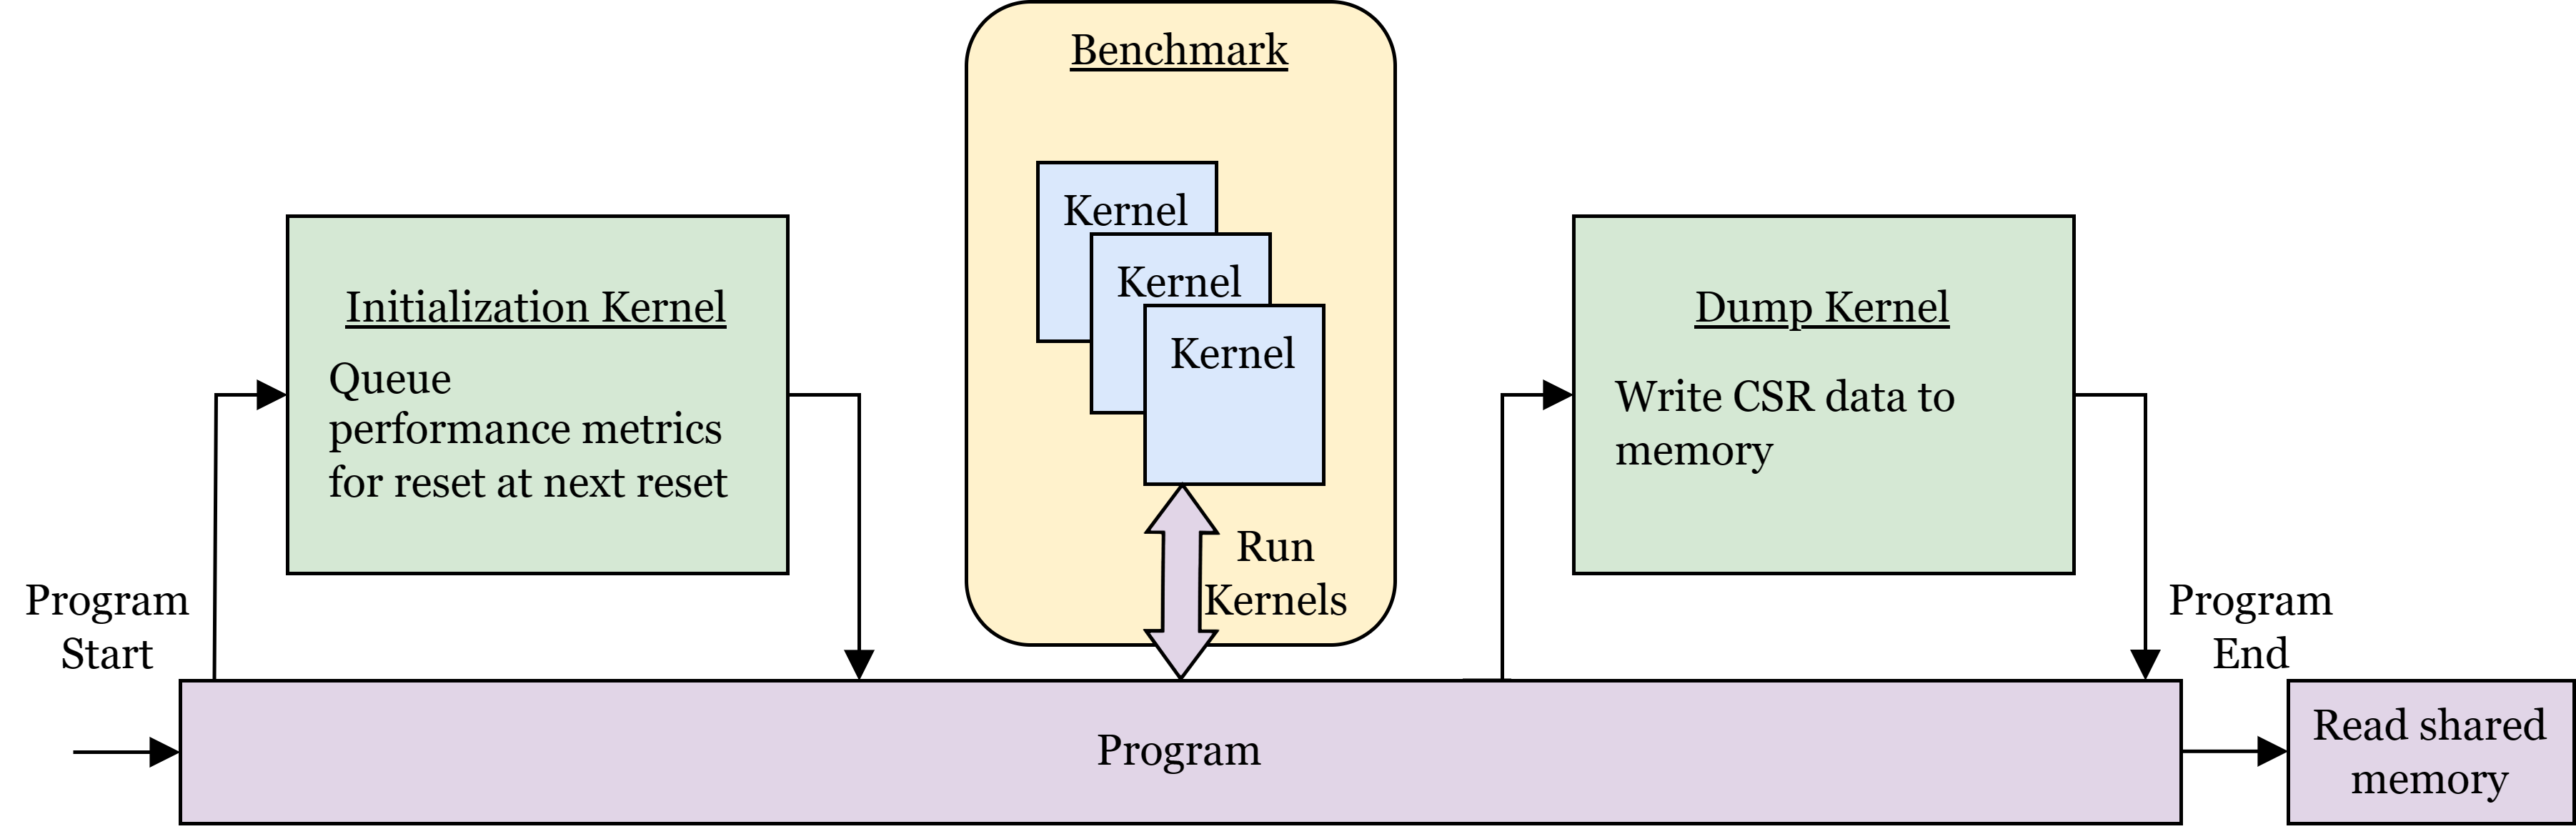
\includegraphics[width=\textwidth]{figures/perf-kernels.png}
    \caption[Illustration of the three stages of multi-kernel benchmarking.]{Illustration of the initialization, run and dump stages of benchmarking. TODO: Numbers, refer to new registers}
    \label{fig:init_run_dump}
\end{figure}

% \textcolor{red}{Init kernel: ensure that the performance metrics are reset at the beginning of the benchmark. This is required as the reset lock register cannot be controlled by anything other than instructions}
% \textcolor{red}{Include in start.S that all kernels start by setting the reset lock, this is only required for the first kernel in the benchmark, but as it is implemented in start.S which is linked to all kernels, every kernel performs the action}
% \textcolor{red}{Dump kernel: ensure that the performance metrics are reset at the beginning of the benchmark}

To make this solution viable to implement for all benchmarks, I created a header containing macros for starting the initialization and dump kernel. To add new benchmarks to \Gls{vortex}, it is only required to include the header and insert the macros for creating and starting the kernels at the correct time. The macros takes the current OpenCL context, command queue and device ID as input. Doing this allowed for more rapid adjustments to the implementation in addition to making the process of adding benchmarks quicker.

% \textcolor{red}{Some of the benchmarks did not run on idun, probably due to compiler differences}

% The existing benchmarks included with \Gls{vortex} are quite simple. They all consist of one kernel which is ran once, while most of the \Gls{rodinia} benchmarks contain multiple kernels. In the current version of Vortex a reset signal is sent to the \acrshort{gpu} before executing a kernel. This resets the GPU, including the registers holding the performance metrics to a known initial state. Thus if a benchmark executes multiple kernels, only the performance metrics of the last kernel persists. 

% As the kernels can have different characteristics, it is ideal to collect performance data for the entire benchmark. To make this possible, we have to stop the performance data from resetting. To achieve this we implemented a \acrfull{plr} which, when high, prevents the performance registers from resetting. This register is a \acrfull{csr} which can be written to using CSR-instructions, and is not affected by reset.

% To initialize the performance metrics, we have to queue a program which clears the \acrshort{plr}. By doing this, the performance metrics can reset before executing the next kernel. All consecutive kernels can set this register high to prevent the parameters from resetting. This allows for collecting performance metrics for the entire benchmark for multi-kernel benchmarks.

% \texttt{Dumping performance metrics at the end of the kernel}

\section{Adapting Benchmarks for Vortex}

The \gls{pocl} driver included with Vortex does not support online compilation of the kernels. Thus all kernels have to be compiled offline and loaded as binaries. This meant that variables could not be passed from the program to the kernel before compilation, but rather had to be set before the offline compilation. Because of this, the benchmarks become less flexible, as some buffer sizes had to be hard-coded before compilation, instead of changing with the input of the benchmark.

While porting \Gls{rodinia} benchmarks to \Gls{vortex}, I observed that the OpenCL functions \textit{clEnqueueNDKernels}, \textit{clEnqueueCopyBuffer} and \textit{clCreateBuffer} sometimes aborted or resulted in segmentation faults. Looking into the cause of the crashes, I found that \textit{clEnqueueNDKernels} caused a segmentation fault when the kernel contained local parameters. It seems like the driver is unable to dynamically allocate local memory for the work-items of the work-groups using \textit{clSetKernelArg}. To solve this, I removed the local parameters of the kernels, and instead defined local buffers in the kernel code. By doing this, the driver does not have to allocate the buffers dynamically. As the size of the local buffers is now defined at compile time of the kernels, I had to hard-code the buffer sizes according with the selected input of the benchmarks.

When benchmarks crashed at \textit{clCreateBuffer}, it was due to the \texttt{GL\_MEM\_ALLOC\_HOST\_PTR} flag of \textit{clCreateBuffer} being set. \texttt{GL\_MEM\_ALLOC\_HOST\_PTR} specifies that the allocated memory should be accessible by the host. To resolve this, I instead created the buffer without the flag, and instead used \texttt{clEnqueueReadBuffer} and \texttt{clEnqueueWriteBuffer} to access the memory whenever needed by the host. This issue is similar to the one above, as it seems to be caused by issues regarding permission to dynamically allocate memory in specific locations.

The last issue I encountered related to OpenCL functions was \textit{clEnqueueCopyBuffer} crashing. \textit{clEnqueueCopyBuffer} copies data from one buffer on the \acrshort{gpu} to another. I is unclear why this does not work, but it could be easily resolved by reading the data from the device to the host using \texttt{clEnqueueReadBuffer}, before writing it back to the correct buffer using \texttt{clEnqueueWriteBuffer}. The workarounds I did to avoid using the problematic OpenCL features should not affect the measured performance, as measurements are made only during kernel execution.

The \textit{Hybridsort} and \textit{Myocyte} benchmarks from \Gls{rodinia} have kernels which required specific functions. This includes \textit{atomic\_add}, \textit{expd}, \textit{powdd} and \textit{sqrtd}. These functions, were missing from the \Gls{pocl} compiler included with \Gls{vortex}. After further inspections, it became apparent that none of the atomic functions are included. Thus these benchmarks could not be included into \Gls{vortex}' benchmark suite.

Table \ref{tab:new_benchmarks} shows the list of Rodinia benchmarks which can execute on \Gls{vortex} after performing the adaptations mentioned in this section. However the benchmarks were not scheduled efficiently, by \Gls{vortex}' static \acrshort{tb} scheduler. The scheduler struggled to divide the work among \Gls{vortex}' \acrshortpl{sm}. For most benchmarks only a small subset of the \acrshortpl{sm} were scheduled any work. Rekdal \cite{Rekdal_Master} encountered the same issue with some of the existing \Gls{vortex} benchmarks. The solution was to reduce the the local work size to 1 when enqueuing the kernels. This reduces the number of work-items per work-group, resulting in more work-groups, which can be scheduled more \acrshortpl{sm}. This method worked to some degree for all benchmarks except \textit{heart wall}, which I was unable to find a solution for.  

% -- Table of benchmarks
\begin{table}
    \centering
    \caption{Rodinia benchmarks added to \Gls{vortex}}
    \begin{tabular}{|l|l|l|l|} 
        \hline
        \textbf{Applications}      & \textbf{Domains} \\ \hhline{|=|=|}
        B+ Tree                    & Graph Traversal \\ \hline
        Back propagation           & Pattern Recognition \\ \hline
        Breadth-First Search       & Graph Algorithms  \\ \hline
        CFD Solver                 & Fluid Dynamics  \\ \hline
        Gaussian elimination       & Linear Algebra \\ \hline
        GPUDWT                     & Image/Video Compression  \\ \hline
        Heart Wall                 & Medical Imaging \\ \hline
        HotSpot                    & Physics Simulation  \\ \hline
        HotSpot3D                  & Physics Simulation  \\ \hline
        Kmeans                     & Data Mining \\ \hline
        LavaMD2                    & Molecular Dynamics\\ \hline
        LU Decomposition           & Linear Algebra  \\ \hline
        Needleman-Wunsch           & Bioinformatics\\ \hline
        Particle Filter            & Medical Imaging \\ \hline
        SRAD                       & Image Processing  \\ \hline
        Streamcluster              & Data Mining \\ \hline
    \end{tabular}
    \label{tab:new_benchmarks}
\end{table}

\section{Fast-Forward, Warm-Up and Early-Exit}

\begin{figure}
    \centering
    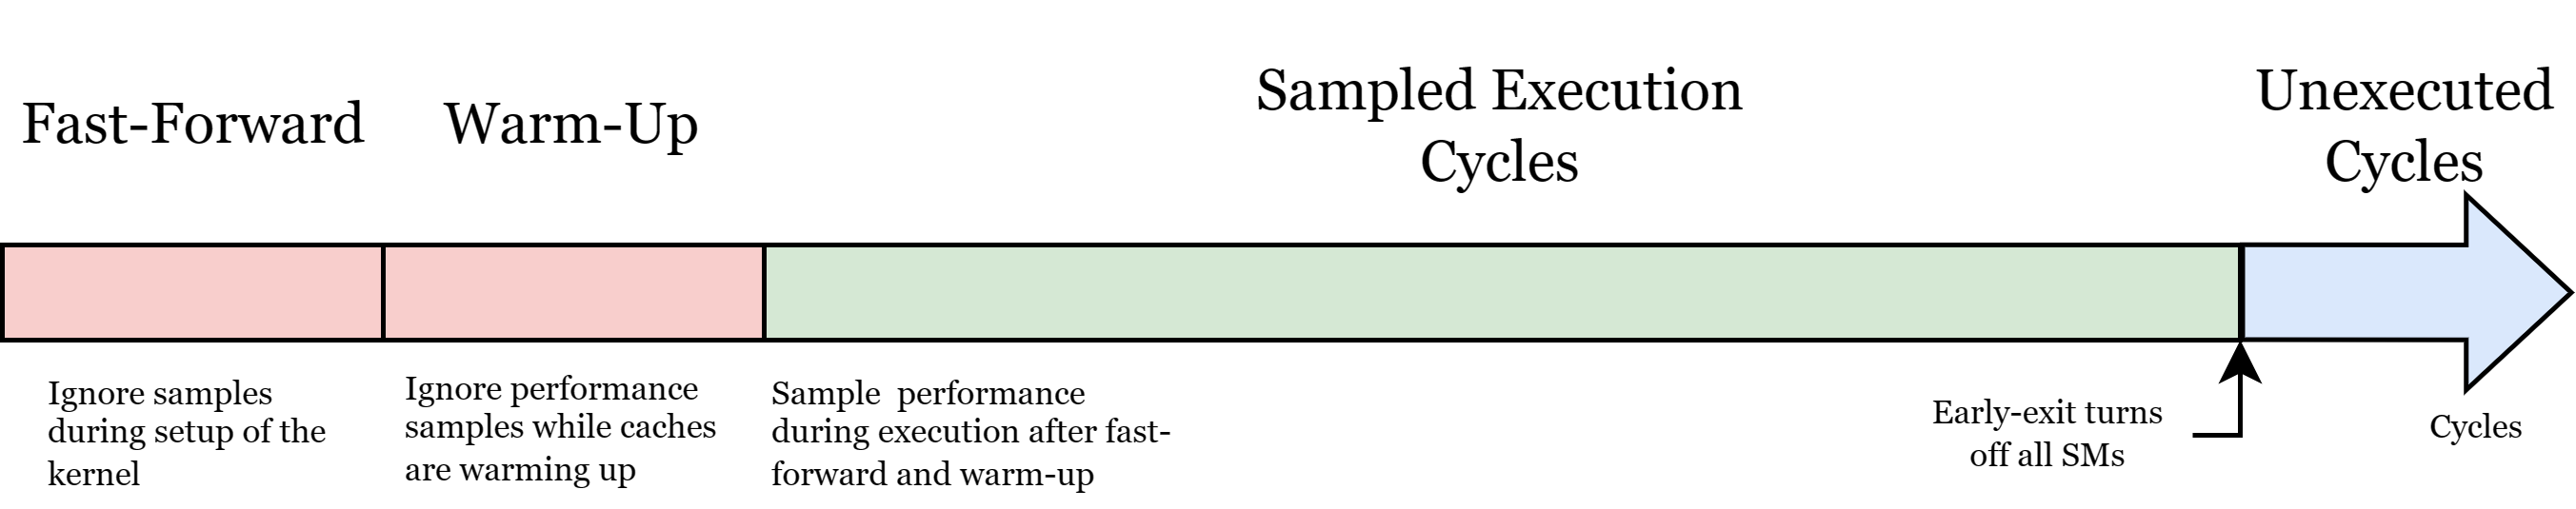
\includegraphics[width=\textwidth]{figures/fast-forward-timeline.png}
    \caption{Timeline explaining \textit{fast-forward, warm-up} and \textit{early-exit}. TODO: Use lock registers}
    \label{fig:ff-timeline}
\end{figure}

Most of the Rodinia benchmarks I added to \Gls{vortex}, require substantially more time to complete execution than the already included benchmarks. When using software simulation, it becomes infeasible to simulate the entire benchmarks, due to long simulation times. One way of solving this would be to reduce the input size, however this would affect the TB scheduler and cache behaviour. A more common approach for reducing simulation time is using \textit{fast-forwarding} and \textit{warm-up} \cite{simpoint}. \textit{Fast-forwarding} is to run a less accurate simulation to a given point in execution, and continue the real simulation from there. This skips over the initialization to an area of the code more representative of the whole benchmark. After \textit{fast-forwarding} using a less accurate simulator, branch predictors and caches will not be in the same state as if an accurate simulation was used. A solution is to run the accurate simulation until the cache hit-rate stabilize before starting to collect performance metrics, this is called \textit{warm-up} and removes the cold-start bias.

There is no emulator or less accurate simulator for \Gls{vortex}, thus \textit{fast-forwarding} and \textit{warm-up} will have limited versatility. To further reduce simulation time, I introduce \textit{early-exit} to \Gls{vortex}. \textit{Early-exit} terminates the benchmark after a given number of cycles. As the number of simulated cycles scales linearly with the simulation time, using \textit{early-exit} allows for easily regulating the simulation time. When implementing \textit{early-exit}, it becomes more important to skip the startup, i.e \textit{fast-forward} and \textit{warm-up}, as it becomes a larger portion of the execution time. 

\textit{Fast-forward} and \textit{warm-up} is implemented by setting the \textit{perf-lock} register, described in Section \ref{sec:reading_perf}, high for a given number of cycles at the beginning of the simulation. Thus no performance data will be collected during the startup. Caches and other components can also be warmed during this period. Note that this is only performed for the first kernel in a benchmark. If a benchmark executes multiple kernels before exiting, the startup cycles become representative of the kernels performance. \textit{Early-exit} is implemented by deactivating all the \acrshortpl{sm} after a number of cycles. This indicates for the driver that \Gls{vortex} has completed its execution. 

This method of implementing \textit{early-exit} is somewhat problematic. When terminating early, the result of the kernels will not be correct. Some of the benchmarks are affected by the results returned by the kernel execution. \textit{Streamcluster} does for example execute the kernel until the result is not getting better. If the result is wrong due to \textit{early-exit}, it might result in an infinite loop of starting and exiting the kernel. To resolve this, I had to manually add safe-guards for \textit{streamcluster} and \textit{kmeans}, setting a maximum number of iterations.

% \textcolor{red}{Benchmarks are too long to run in software simulation, introduce early exit and warp-up. How was this implemented in vortex}

% \textcolor{red}{When implementing early exit, a problem arose, some benchmarks had exit conditions based on the result of their kernel. When using early exit, the result data my be garbage and result in infinite loops. To resolve this each benchmark had to be inspected to find loops and branches with conditions based on the kernel results and add safeguards, such as max number of iterations}

% \section{Cactus}

% \textcolor{red}{This could possibly be related work:}

% \textcolor{red}{Cactus vs Rodina, problematic to implement too many kernels. Rodinia is nice, because it usually between 1 and 3 kernels, easier to capture the behaviour when using software simulation, as the benchmarks cannot run long enough to capture behaviour from all kernels}